\documentclass{article}
\usepackage{geometry}
\geometry{a4paper, margin=1in}
\usepackage{graphicx}
\usepackage[colorlinks=true, linkcolor=blue, citecolor=blue, urlcolor=blue]{hyperref}
\usepackage{listings}
\usepackage{xcolor}
\usepackage{amsmath}
\usepackage{enumitem}
\usepackage{float}

\lstset{
    language=NASM,
    basicstyle=\ttfamily\footnotesize\selectfont, % use the selected monospaced font
    backgroundcolor=\color{white},
    keywordstyle=\color{blue},
    commentstyle=\color{gray},
    stringstyle=\color{red},
    numbers=left,
    numberstyle=\tiny\color{gray},
    stepnumber=1,
    numbersep=10pt,
    frame=single,
    breaklines=true,
    captionpos=b,
    tabsize=4
}

\title{Assignment 6: DOS Virus via IVT+VRAM}
\author{
    [Welby Seely] \\
    \texttt{[wseely@emich.edu]}
}
\date{\today}

\begin{document}

    \maketitle
    \section{Overview}\label{sec:intro}
    The bootloader was heavily updated:

    \begin{itemize}
        \item Switched back to VGA Graphics Mode
        \item Reintroduced the giant `W' bitmap.
        \item Rewrote the custom interrupt services to operate in VGA Graphics Mode
        \begin{itemize}
            \item Sourcing the font is what probably took the most time.
        \end{itemize}
        \item Updated the custom interrupt services to act as a `virus'.
        \begin{itemize}
            \item Overrode Interrupt 10H Service 6 for clearing the screen
            \begin{itemize}
                \item It now prints out the 256 available VGA colors as a background.
            \end{itemize}
            \item Overrode Interrupt 10H Service 19 : Write character string
            \begin{itemize}
                \item It now randomly garbles the pixel color data of the rendered text while retaining the glyphs (so it\textsc{\char13}s still readable).
            \end{itemize}
        \end{itemize}
    \end{itemize}

    \section{The Virus}\label{sec:virus}
    The code for the virus is located in logical sector 41 as per requirements, and is loaded to linear address 0x7e00 in memory.

    Getting a pointer to the font was difficult.
    Interrupt 10H Service 17 : Character Generator subservice 30h was used to retrieve the font of the 8 x 8 double-dot font pointer.
    This was then copied to a buffer in memory at linear address 0x9000 for later use by the `virus'.
    Copying was necessary because the region of memory pointed to by the 03h pointer was seemingly shadowed in VGA Graphics mode, so I copied it into a buffer for later use before switching to VGA Graphics mode.

    A custom print function was then implemented to write the font glyphs to the VGA memory-mapped I/O at segment 0xA000.
    Random values were used for the text pixel color to give the text a `virusy' look.

    Similarly, the custom clear function was updated to iterate through the 256 color palate for the background colors.

    \section{Screenshots}\label{sec:screenshots}
    Screenshots of the splash screen and the prompt screen are provided from both Dosbox and from a vintage Packard Bell 486.

    \begin{figure}[H]  % [H] forces the figure to appear here
        \centering
        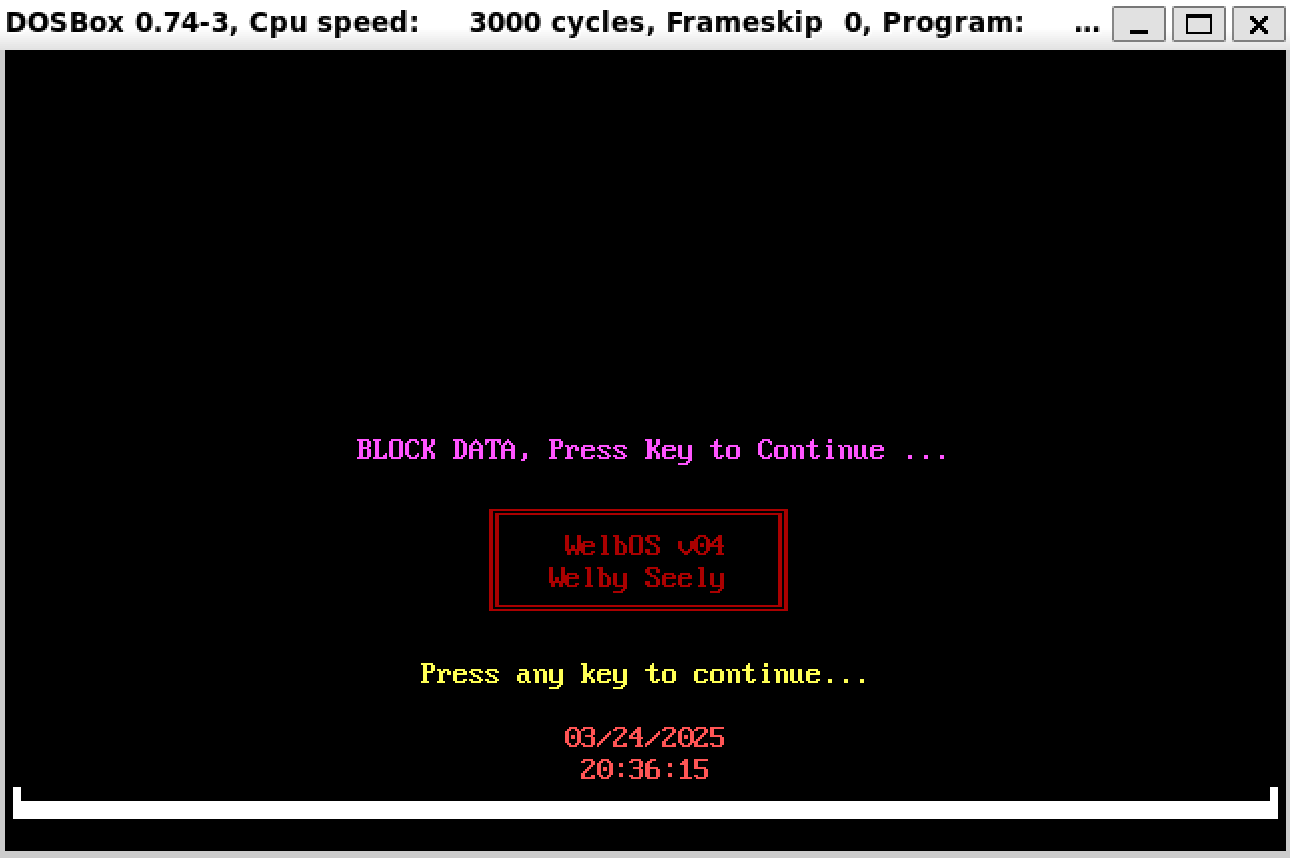
\includegraphics[width=\textwidth]{splash-screen} % Scales image to document width
        \caption{Virus-Infected Custom VGA Graphics Splash Screen}
        \label{fig:1}
    \end{figure}

    \begin{figure}[H]  % Ensures figure appears right here
        \centering
        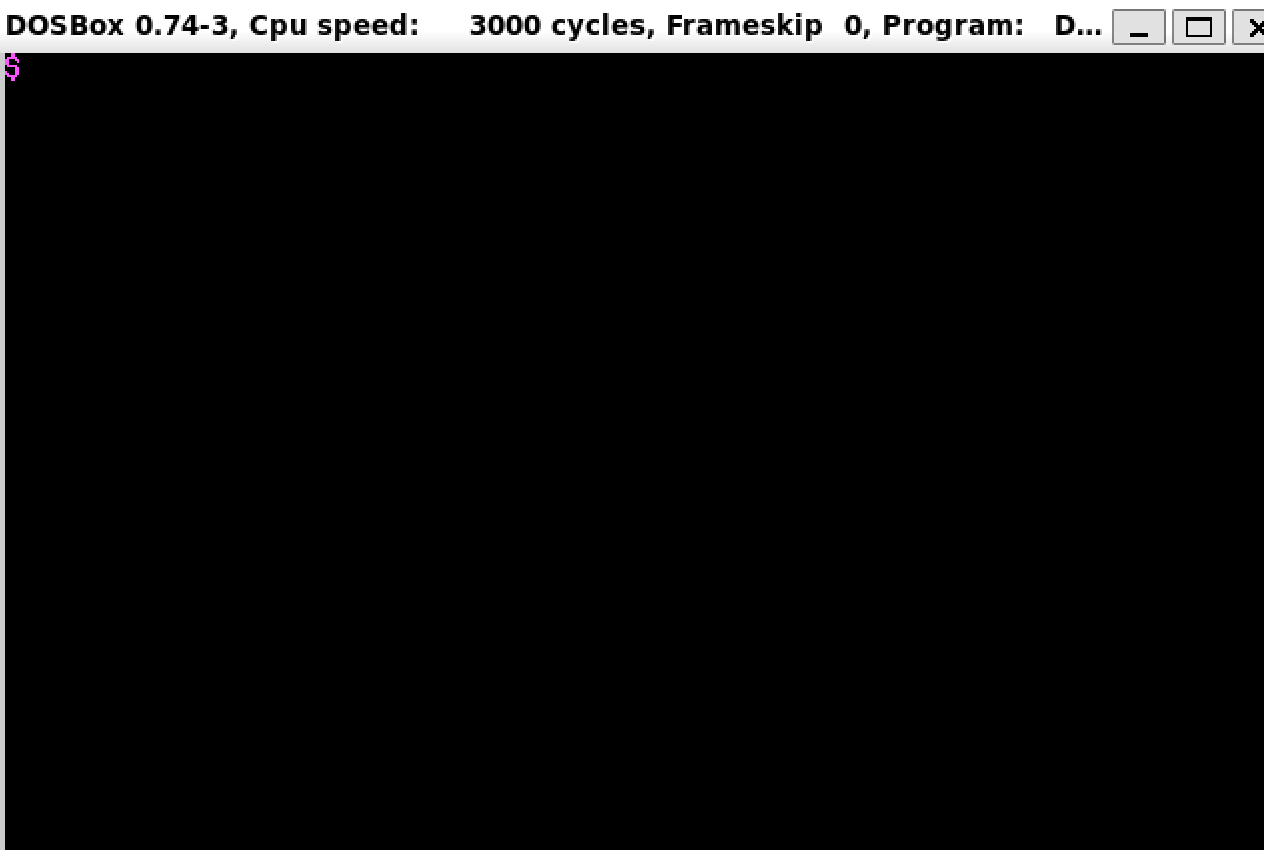
\includegraphics[width=\textwidth]{prompt} % Scales image to document width
        \caption{Virus-Infected Prompt Screen (Rainbow is from the Clear Function)}
        \label{fig:2}
    \end{figure}

    \begin{figure}[H]
        \centering
        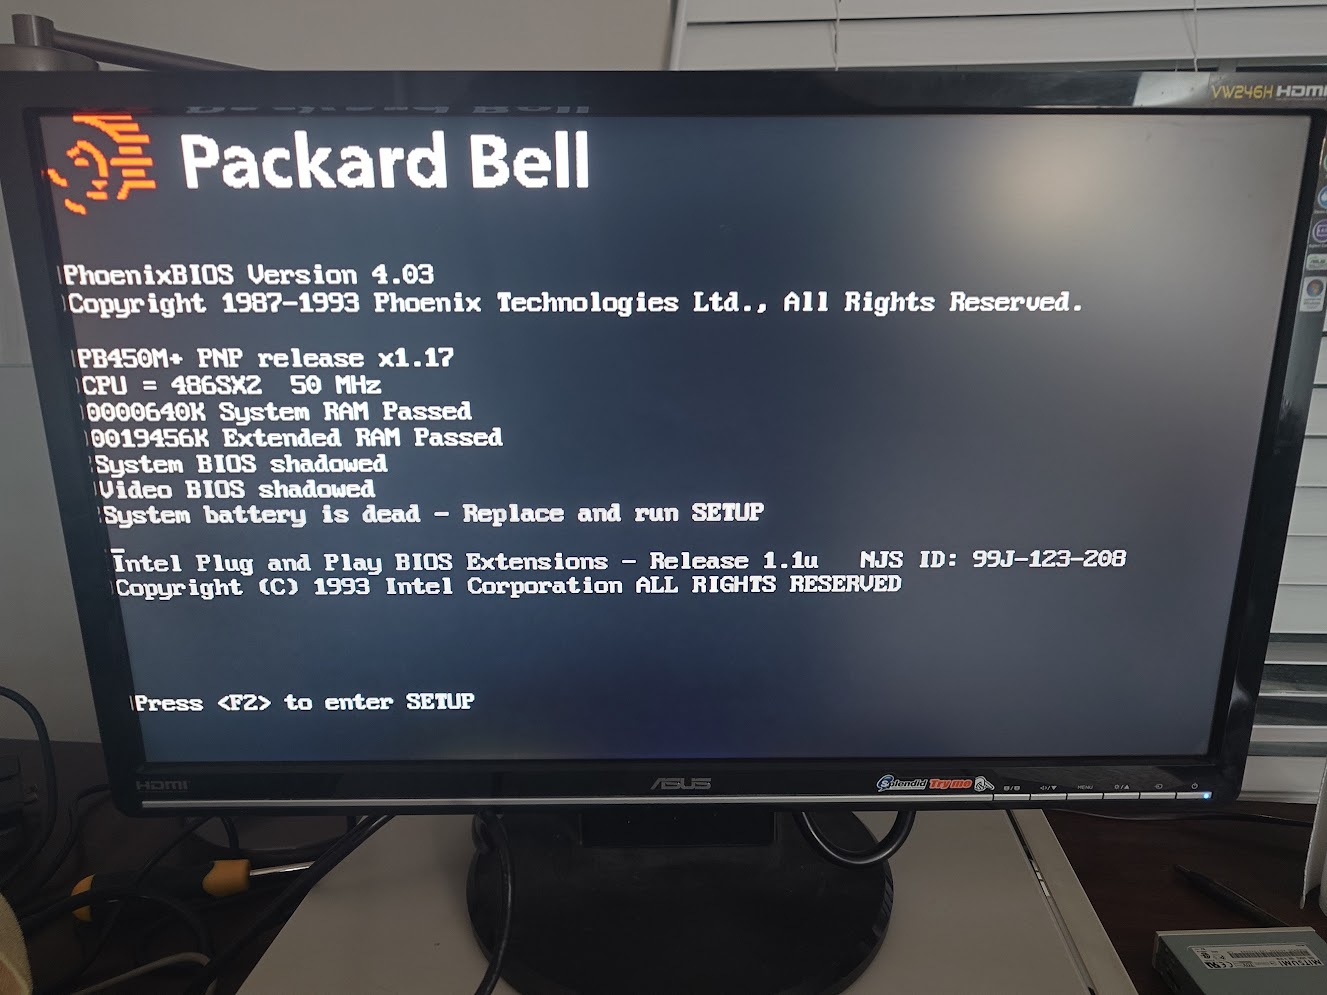
\includegraphics[width=\textwidth]{packard-bell} % Scales image to document width
        \caption{Booting Up the Computer of My Childhood (I need to Replace the CMOS Battery!)}
        \label{fig:3}
    \end{figure}

    \begin{figure}[H]
        \centering
        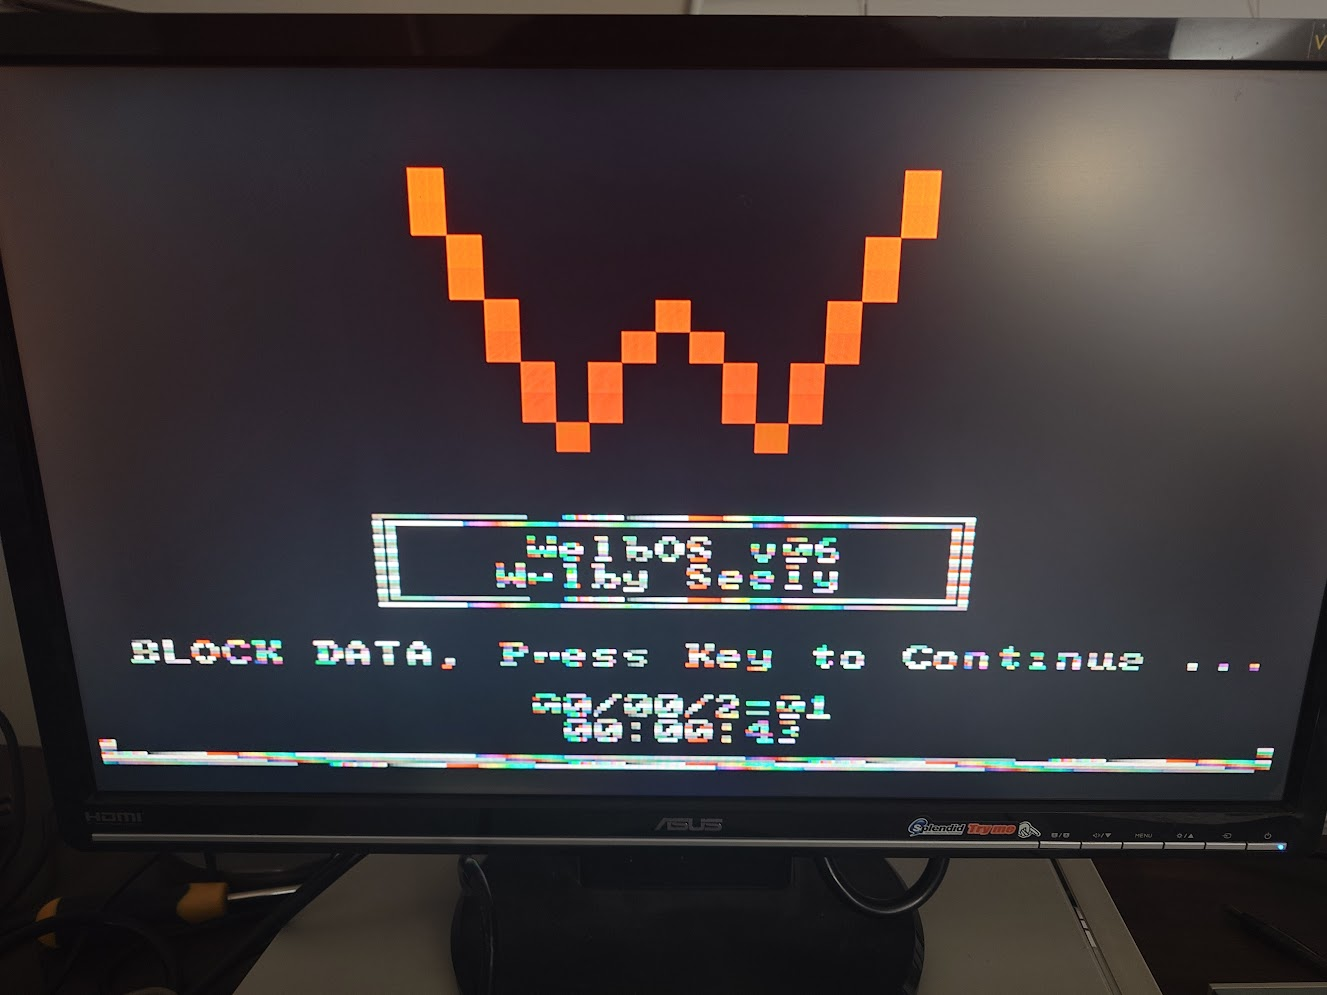
\includegraphics[width=\textwidth]{packard-splash} % Scales image to document width
        \caption{Virus-Infected 486 Splash Screen - Note the Dead Clock}
        \label{fig:4}
    \end{figure}

    \begin{figure}[H]
        \centering
        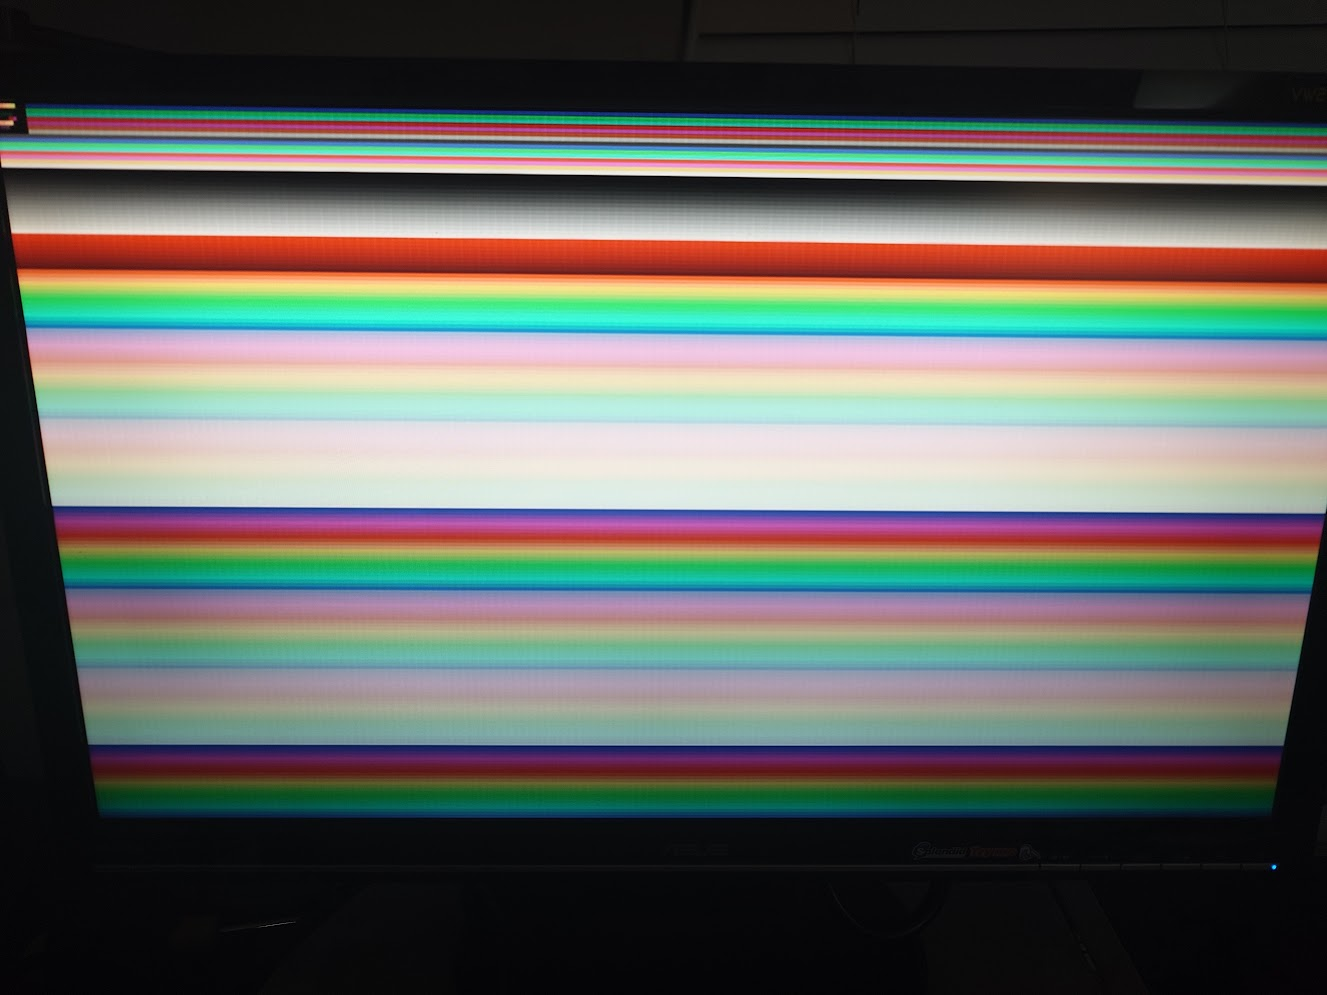
\includegraphics[width=\textwidth]{packard-prompt} % Scales image to document width
        \caption{Virus-Infected 486 Prompt Screen}
        \label{fig:5}
    \end{figure}

    \section{Appendix 1: Source Code}\label{sec:appendix_1}
    \begin{lstlisting}[caption={os623V06.asm listing}, captionpos=t]
        bits 16
        BIOS_VIDEO          equ 0x10
        DISPLAY_FUN         equ 0x13
        CLEAR_FUN           equ 0x06

        FUN_VIDEO_MODE      equ 0x0000
        VGA_MODE            equ 0x0013

        BIOS_FLOPPY         equ 0x0013
        READ_SECTORS        equ 0x0002

        ; ext code
        MAIN_SEG equ 0x0001
        MAIN_OFF equ 0x2345

        STRING_SEG equ 0x0001
        STRING_OFF equ 0x7890

        MAGENTA_BLACK equ 0x0D
        YELLOW_BLACK        equ 0x0E

        VGA_DISPLAY_WIDTH   equ 320
        VGA_DISPLAY_HEIGHT  equ 200

        VIRUS_SEG            equ 0
        VIRUS_OFF            equ 0x7e00

        RED_BLACK           equ 0x04
        FONT_BUFFER         equ 0x9000


        ; 1) attribute
        ; 2) length of string
        ; 3) segment of string
        ; 4) address of string
        ; 5) row position
        ; 6) column position
        %macro PRINT 6
            mov bl, %1         ; Attribute
            mov cx, %2         ; length of the string
            mov ax, %3         ; segment of the string
            mov es, ax
            mov bp, %4         ; address of the string
            mov dh, %5         ; row position
            mov dl, %6         ; column position

            mov  ah, DISPLAY_FUN    ; BIOS display string (function 13h)
            mov  al, 0              ; Write mode = 1 (cursor stays after last char
            mov  bh, 0              ; Video page
            int  BIOS_VIDEO
        %endmacro

        org 0x7c00
        jmp short start
        nop

        bsOEM       db "WelbOS v06"         ; OEM String

        start:

            call configure_video
            call set_ivt

            ; Inputs: cylinder, sector, head, segment, offset.
            push 1
            push 6
            push 0
            push VIRUS_SEG
            push VIRUS_OFF
            call 0x:load_sector
            ; Inputs: cylinder, sector, head, segment, offset.
            push 1
            push 2
            push 0
            push MAIN_SEG
            push MAIN_OFF
            call 0x:load_sector

            call MAIN_SEG:MAIN_OFF

            ; Inputs: cylinder, sector, head, segment, offset.
            push 0
            push 2
            push 0
            push 0x0001
            push 0x7890
            call 0x:load_sector

            PRINT YELLOW_BLACK, 37, 0x0001, 0x7890, 19, 2

            ; Wait for key press
            mov ah, 0x00
            int 0x16

            push cs
            pop ds

            mov ah, CLEAR_FUN
            int BIOS_VIDEO

            mov ax, 0x0003
            int BIOS_VIDEO

            push MAGENTA_BLACK
            push 1
            push prompt_sym
            push 0
            push 0
            call 0x:print

            call set_cursor_pos

            jmp $

        times 0xD0 - ($ - $$) db 0

        ; -----------------------------------------------------------------------------
        ; Function: print
        ; Description: Prints a string to the console.
        ; Inputs:
        ;   - [bp+6] Column position to begin writing the string.
        ;   - [bp+8] Row position to begin writing the string.
        ;   - [bp+10] Memory address location of the string.
        ;   - [bp+12] Length of the string.
        ;   - [bp+14] Attribute.
        ; Outputs: None.
        ; Modifies:
        ;   - AX, BX, CX, DX, VGA text buffer section (0xB800)

        ; -----------------------------------------------------------------------------
        print:
            push bp
            mov bp, sp
            mov bl, [bp+14]        ; Attribute (lightgreen on black)
            mov cx, [bp+12]        ; length of the string
            push ds
            pop es                 ; segment of the string
            mov dh, [bp+8]         ; row position
            mov dl, [bp+6]         ; column position
            mov bp, [bp+10]        ; address of the string, !!destructive to relative frame refs!!

            mov  ah, 13h            ; BIOS display string (function 13h)
            mov  al, 0              ; Write mode = 1 (cursor stays after last char
            mov  bh, 0              ; Video page
            int BIOS_VIDEO

            pop bp
            retf 10

        times 0x180 - ($ - $$) db 0

        ; -----------------------------------------------------------------------------
        ; Function: load_sector
        ; Description: Loads a sector into memory
        ; Inputs: cylinder, sector, head, segment, offset.
        ; Outputs: 512 bytes into memory as specified by segment and offset.
        ; Note: Does not currently take into account all 10 bits of the cylinder.
        ; Modifies:
        ;   - AX, BX, CX, DX, EX
        ; Calls:
        ;   - BIOS interrupt 0x13, function 0x02.
        ; -----------------------------------------------------------------------------
        load_sector:
            push bp
            mov bp, sp

            mov bx, [bp + 8]            ; segment (can't move immediate into segment register)
            mov es, bx                  ; segment
            mov bx, [bp + 6]            ; offset
            mov ah, READ_SECTORS        ; function
            mov al, 1                   ; number of sectors to read
            mov ch, [bp + 14]           ; cylinder number (10 bits, upper two bits are 6 and 7 of CL)
            mov cl, [bp + 12]           ; sector number (and upper two of cylinder)
            mov dh, [bp + 10]           ; head (usually same as side)
            mov dl, 0                   ; drive number
            int BIOS_FLOPPY

            pop bp
            retf 10

        set_cursor_pos:
            mov ah, 0x01          ; BIOS Set Cursor Shape function
            mov ch, 0x06          ; Start scan line
            mov cl, 0x07          ; End scan line
            int BIOS_VIDEO        ; BIOS video interrupt

            mov ah, 0x02        ; BIOS function: set cursor position
            mov bh, 0x00        ; Page number (0)
            mov dh, 0x00        ; Row (0)
            mov dl, 0x01        ; Column (1)
            int BIOS_VIDEO
            ret

        set_ivt:
            push ax
            push es

            xor ax, ax
            mov es, ax                                           ; es = 0x0000, IVT segment
            cli                                                  ; disable interrupts during change
            mov word [es:BIOS_VIDEO * 4], VIRUS_OFF            ; IP for int 0xf0 → point to `function_group`
            mov   word [es:BIOS_VIDEO * 4 + 2 ], cs            ; CS for int 0xf0 → current segment
            sti                                                  ; re-enable interrupts

            pop es
            pop ax
            ret

        configure_video:
            ; set text mode to get font
            mov ax, 0x0003
            int BIOS_VIDEO

            ; get font pointer
            mov ax, 0x1130
            mov bh, 0x03
            int BIOS_VIDEO

            ; move into a font buffer
            ; source font
            push es
            pop ds
            mov si, bp
            ; destination buffer
            mov ax, 0
            mov es, ax
            mov di, FONT_BUFFER
            mov cx, 256 * 8
            cld
            rep movsb

            ; reset ds (set to 0 stored in ax)
            mov ds, ax

            mov ax, FUN_VIDEO_MODE + VGA_MODE
            int BIOS_VIDEO
            ret

        prompt_sym          db "$"

        ; Pad to 512 bytes for an MBR:
        padding times 510 - ($ - $$) db 0

        ; Optional boot signature:
        bootSig db 0x55, 0xAA
    \end{lstlisting}
    \begin{lstlisting}[caption={loaderV06.asm listing}, captionpos=t]
        bits 16
        BIOS_VIDEO          equ 0x10
        DISPLAY_FUN         equ 0x13

        FUN_VIDEO_MODE      equ 0x0000
        VGA_MODE            equ 0x0003

        BIOS_FLOPPY         equ 0x0013
        READ_SECTORS        equ 0x0002

        VGA_DISPLAY_WIDTH   equ 320
        DISPLAY_WIDTH       equ 40
        DISPLAY_HEIGHT      equ 25
        VGA_TXT_DISP_WIDTH  equ 40
        VGA_TXT_DISP_HEIGHT equ 25
        MESSAGE_ROW         equ VGA_TXT_DISP_HEIGHT / 2 + 3
        LINE_ROW_TOP        equ MESSAGE_ROW - 1
        LINE_ROW_NAME       equ MESSAGE_ROW + 1
        LINE_ROW_BOTTOM     equ LINE_ROW_NAME + 1
        LINE_ROW_ANYKEY     equ LINE_ROW_BOTTOM + 2
        TEXT_MODE           equ 0x03
        MAGENTA_BLACK       equ 0x0D
        WHITE_BLACK         equ 0x0F
        RED_BLACK           equ 0x04
        YELLOW_BLACK        equ 0x0E

        BOX_LENGTH          equ 19
        ANYKEY_LENGTH       equ 28
        BITMAP_LENGTH       equ 18
        SHADE_COUNT         equ 9

        SCALING_FACTOR      equ 0x8
        LOGO_START_X        equ (VGA_DISPLAY_WIDTH - (16 * SCALING_FACTOR)) / 2
        LOGO_START_Y        equ (200 - (9 * SCALING_FACTOR)) / 2 -40

        PRINT_SEGMENT       equ 0
        PRINT_OFFSET        equ 0x7cD0

        LOAD_SECTOR_SEGMENT equ 0
        LOAD_SECTOR_OFFSET  equ 0x7d60

        DISPLAY_TIME_SEGMENT equ 0x0002
        DISPLAY_TIME_OFFSET  equ 0x3456

        %define CENTER_TXT(len) ((DISPLAY_WIDTH - len) / 2)
        %define CENTER_VGA_TXT(len) ((VGA_TXT_DISP_WIDTH - len) / 2)

        org 0x2345
        main:
            push ds
            push cs
            pop ds

        hide_cursor:
            mov ah, 0x01          ; BIOS Set Cursor Shape function
            mov ch, 0b00001000    ; Start scan line (set bit 5 to hide cursor)
            mov cl, 0x00          ; End scan line (N/A)
            int BIOS_VIDEO        ; BIOS video interrupt

        palette:
            call set_red_gradient_palette
        load_time:
            push 1
            push 5
            push 0
            push DISPLAY_TIME_SEGMENT
            push DISPLAY_TIME_OFFSET
            call LOAD_SECTOR_SEGMENT:LOAD_SECTOR_OFFSET

            push RED_BLACK
            push BOX_LENGTH
            push welbos
            push MESSAGE_ROW
            push CENTER_VGA_TXT(BOX_LENGTH)
            call PRINT_SEGMENT:PRINT_OFFSET

            push RED_BLACK
            push BOX_LENGTH - 1               ; Repeat count
            push CENTER_VGA_TXT(BOX_LENGTH)   ; Column
            push LINE_ROW_TOP                 ; Row
            push topline                      ; Address of 3-tuple
            call draw_line

            push RED_BLACK
            push BOX_LENGTH
            push name
            push LINE_ROW_NAME
            push CENTER_VGA_TXT(BOX_LENGTH)
            call PRINT_SEGMENT:PRINT_OFFSET

            push RED_BLACK
            push BOX_LENGTH - 1       ; Repeat count
            push CENTER_VGA_TXT(BOX_LENGTH)   ; Column
            push LINE_ROW_BOTTOM     ; Row
            push bottomline             ; Address of 3-tuple
            call draw_line

            push WHITE_BLACK
            push VGA_TXT_DISP_WIDTH - 1       ; Repeat count
            push 0   ; Column
            push LINE_ROW_ANYKEY + 4          ; Row
            push blockline                    ; Address of 3-tuple
            call draw_line

            push LOGO_START_X
            push LOGO_START_Y
            call draw_logo

        show_time:
            call DISPLAY_TIME_SEGMENT:DISPLAY_TIME_OFFSET

            pop ds
            retf

        draw_line:
            push bp
            mov bp, sp

            ;left edge
            push word [bp + 12]
            push 1
            mov si, [bp + 4]
            push si
            mov si, [bp + 6]
            push si
            mov si, [bp + 8]
            push si
            call PRINT_SEGMENT:PRINT_OFFSET

            ; set up middle loop
            mov ax, 1                           ; break when == to cx
        draw_line_middle:
            mov cx, [bp + 10]
            cmp ax, cx
            je draw_line_right
            push ax

            push word [bp + 12]
            push 1
            mov si, [bp + 4]
            inc si
            push si
            mov si, [bp + 6]
            push si
            mov si, [bp + 8]
            add si, ax
            push si
            call PRINT_SEGMENT:PRINT_OFFSET

            pop ax
            inc ax
            jmp draw_line_middle

        draw_line_right:
            push word [bp + 12]
            push 1
            mov si, [bp + 4]
            add si, 2
            push si
            mov si, [bp + 6]
            push si
            add ax, [bp + 8]                    ; rightmostposition
            push ax
            call PRINT_SEGMENT:PRINT_OFFSET

            pop bp
            ret 10

        draw_logo:
            push bp
            mov bp, sp

            mov ax, [bp + 4]
            mov cx, VGA_DISPLAY_WIDTH
            mul cx
            add ax, [bp + 6]
            mov di, ax

            mov ax, 0xA000     ; memory mapped I/O segment for VGA
            mov es, ax

            mov si, w_bitmap   ; source bitmap start address

            mov dx, 9                  ; logical row that we're calculating
            push SCALING_FACTOR
        .draw_rows:
            mov bx, 9
            sub bx, dx                 ; determine color for this row
            mov bl, [row_colors + bx]  ; store row color in BL (or AL, but we’ll need AL soon)
            mov ax, [si]               ; retrieve pixels for this row

            ; Process 16 pixels
            mov cx, 16
        .draw_row:
            shl ax, 1          ; Shift left (test MSB of AX)
            jnc .skip_column

            push cx
            push ax
            mov cx, SCALING_FACTOR
            mov al, bl
            rep stosb
            pop ax
            pop cx
            jmp .next_column
        .skip_column:
            add di, SCALING_FACTOR
        .next_column:
            loop .draw_row

        .scale_vertically:
            add di, 320 - 16 * SCALING_FACTOR ; Move to next VGA row
            pop cx
            dec cx
            cmp cx, 0
            jz .next_source_row
            push cx
            jmp .draw_rows
        .next_source_row:
            add si, 2
            dec dx
            jz .next_color
            push SCALING_FACTOR
            jmp .draw_rows
        .next_color:
            pop bp
            ret 4

        set_red_gradient_palette:
            mov dx, 0x3C8   ; VGA color index port
            mov al, 32      ; Start setting colors from index 32
            out dx, al
            inc dx          ; Now dx = 0x3C9 (RGB color data port)

            mov cx, 9       ; 9 shades for 9 rows
            mov si, red_shades
        .next_color:
            mov al, [si]    ; Load Red intensity
            out dx, al      ; Set Red value
            xor al, al      ; Set Green=0
            out dx, al
            out dx, al      ; Set Blue=0
            inc si
            loop .next_color
            ret

        topline             db 0xC9
                            db 0xCD
                            db 0xBB
        bottomline          db 0xC8
                            db 0xCD
                            db 0xBC
        blockline           db 0xDE
                            db 0xDC
                            db 0xDD
        welbos              db 0xBA, `    WelbOS v06   `, 0xBA
        welboslen           equ ($ - welbos)
        name                db 0xBA, `   Welby Seely   `, 0xBA
        namelen             equ ($ - name)
        anykey              db "Press any key to continue..."
        anykeylen           equ ($ - anykey)
        red_shades db 58, 55, 50, 45, 40, 35, 30, 25, 20; Bright to dark red
        ; Row color table, from top to bottom row
        row_colors db 32, 33, 34, 35, 36, 37, 38, 39, 40  ; Use only custom red shades
        w_bitmap db 02h, 80h
                 db 02h, 80h
                 db 04h, 40h
                 db 04h, 40h
                 db 08h, 21h
                 db 88h, 22h
                 db 50h, 14h
                 db 50h, 14h
                 db 20h, 08h
    \end{lstlisting}
    \begin{lstlisting}[caption={datetimeV06.asm listing}, captionpos=t]
        PRINT_SEGMENT       equ 0
        PRINT_OFFSET        equ 0x7cA0

        VGA_TXT_DISP_HEIGHT equ 25
        VGA_TXT_DISP_WIDTH  equ 40

        MESSAGE_ROW         equ VGA_TXT_DISP_HEIGHT / 2 + 3
        LINE_ROW_TOP        equ MESSAGE_ROW - 1
        LINE_ROW_NAME       equ MESSAGE_ROW + 1
        LINE_ROW_BOTTOM     equ LINE_ROW_NAME + 1
        LINE_ROW_ANYKEY     equ LINE_ROW_BOTTOM + 2
        LIGHT_RED           equ 0x0C

        %macro makedt 4
            mov bh,%1 			;dh/dl/chcl
            shr bh,4
            add bh,30h 			;add 30h to convert to ascii
            mov [%2 + %3],bh
            mov bh,%1
            and bh,0fh
            add bh,30h
            mov [%2 + %4],bh
        %endmacro

        %define CENTER_VGA_TXT(len) ((VGA_TXT_DISP_WIDTH - len) / 2)

        bit16
        org 0x3456

            push ds
            push cs
            pop ds

            mov ah,04h	 ;function 04h (get RTC date)
            int 1Ah		;BIOS Interrupt 1Ah (Read Real Time Clock)

            makedt dh, dtfld, 0, 1  ; month
            makedt dl, dtfld, 3, 4  ; day
            makedt ch, dtfld, 6, 7  ; century
            makedt cl, dtfld, 8, 9  ; year

            mov ah,02h
            int 1Ah

            makedt ch, tmfld, 0, 1  ; hours
            makedt cl, tmfld, 3, 4  ; minutes
            makedt dh, tmfld, 6, 7  ; seconds

            push LIGHT_RED
            push 10
            push dtfld
            push LINE_ROW_ANYKEY + 2
            push CENTER_VGA_TXT(10)
            call PRINT_SEGMENT:PRINT_OFFSET

            push LIGHT_RED
            push 8
            push tmfld
            push LINE_ROW_ANYKEY + 3
            push CENTER_VGA_TXT(8)
            call PRINT_SEGMENT:PRINT_OFFSET

            pop ds
            retf

        dtfld: db '00/00/0000'
        tmfld: db '00:00:00'
    \end{lstlisting}
    \begin{lstlisting}[caption={virusV06.asm listing}, captionpos=t]
        DISPLAY_FUN         equ 0x13
        CLEAR_FUN           equ 0x06

        VGA_DISPLAY_WIDTH   equ 320
        VGA_DISPLAY_HEIGHT  equ 200
        FONT_OFFSET         equ 0x9000
        FONT_SEGMENT        equ 0x0
        FONT_SIZE           equ 8
        VGA_SEGMENT         equ 0xA000

        bits 16
        org 0x7e00

        function_group:
          cmp ah, DISPLAY_FUN
          je .disp
          cmp ah, CLEAR_FUN
          je .clear_screen
          jmp .end

        ; -----------------------------------------------------------------------------
        ; Function: disp - Print string using font at FONT_OFFSET
        ; Parameters:
        ;    bl         ; Foreground color
        ;    cx         ; String length
        ;    es:bp      ; String address
        ;    dh         ; Row (character position)
        ;    dl         ; Column (character position)
        ; -----------------------------------------------------------------------------
        .disp:
            push ds
            push bx
            push si
            push di

            ; Set font and VGA segments
            mov ax, FONT_SEGMENT
            mov fs, ax
            mov ax, VGA_SEGMENT
            mov ds, ax

            ; Calculate initial pixel offset (di)
            movzx ax, dh                            ; row
            imul ax, VGA_DISPLAY_WIDTH * FONT_SIZE  ; row * 320*FONT_SIZE
            movzx dx, dl                            ; column
            shl dx, 3                               ; column * 8 (FONT_SIZE)
            add ax, dx
            mov di, ax                              ; di = starting offset

            mov bx, di                              ; Save base position in bx
            mov si, bp                              ; es:si = string address

        .draw_char_loop:
            jcxz .end_draw                ; end when cx=0

            ; Load character and get font data
            mov al, [es:si]
            inc si
            movzx di, al
            shl di, 3
            add di, FONT_OFFSET           ; fs:di = font data

            ; Draw 8 rows
            push cx
            mov cx, FONT_SIZE
        .draw_row:
            push cx
            mov al, [fs:di]               ; font byte for current row
            inc di

            ; Draw 8 bits (pixels)
            mov cx, FONT_SIZE
            mov ah, al                    ; copy font byte to ah
        .draw_bit:
            shl ah, 1                     ; draw highest bit
            mov al, 0                     ; default background (black)
            jnc .skip_foreground          ; Test highest big (don't draw if 0)
            mov al, bl                    ; we're using bx for the loop, so let's use this as a random value for the "virus"
        .skip_foreground:
            mov [ds:bx], al
            inc bx                        ; Next pixel column
            loop .draw_bit

            ; Move to next row (bx += 320 - 8)
            add bx, VGA_DISPLAY_WIDTH - FONT_SIZE
            pop cx
            loop .draw_row

            ; Restore bx to next character's base (current bx is at start + 320*8)
            sub bx, (VGA_DISPLAY_WIDTH * FONT_SIZE) - FONT_SIZE
            pop cx
            dec cx
            jmp .draw_char_loop

        .end_draw:
            pop di
            pop si
            pop bx
            pop ds
            jmp .end

        .clear_screen:
            mov ax, VGA_SEGMENT
            mov es, ax
            xor di, di
            mov dx, VGA_DISPLAY_HEIGHT
            mov al, 0x0 ; we'll iterate through our colors
        .clear_row:
            mov cx, VGA_DISPLAY_WIDTH
            rep stosb
            inc al
            dec dx
            jne .clear_row
        .end:
            iret
    \end{lstlisting}
    \begin{lstlisting}[caption={stringV06.asm listing}, captionpos=t]
        db 'BLOCK DATA, Press Key to Continue ...'
    \end{lstlisting}
    \end{document}
